\documentclass[14pt]{extbook}
\usepackage{multicol, enumerate, enumitem, hyperref, color, soul, setspace, parskip, fancyhdr} %General Packages
\usepackage{amssymb, amsthm, amsmath, bbm, latexsym, units, mathtools} %Math Packages
\everymath{\displaystyle} %All math in Display Style
% Packages with additional options
\usepackage[headsep=0.5cm,headheight=12pt, left=1 in,right= 1 in,top= 1 in,bottom= 1 in]{geometry}
\usepackage[usenames,dvipsnames]{xcolor}
\usepackage{dashrule}  % Package to use the command below to create lines between items
\newcommand{\litem}[1]{\item#1\hspace*{-1cm}\rule{\textwidth}{0.4pt}}
\pagestyle{fancy}
\lhead{Makeup Progress Quiz -1}
\chead{}
\rhead{Version B}
\lfoot{7547-2949}
\cfoot{}
\rfoot{Fall 2020}
\begin{document}

\begin{enumerate}
\litem{
Solve the quadratic equation below. Then, choose the intervals that the solutions belong to, with $x_1 \leq x_2$ (if they exist).\[ 15x^{2} +9 x -7 = 0 \]\begin{enumerate}[label=\Alph*.]
\item \( x_1 \in [-2.42, -0.9] \text{ and } x_2 \in [0.02, 0.96] \)
\item \( x_1 \in [-0.56, 0.21] \text{ and } x_2 \in [0.94, 1.53] \)
\item \( x_1 \in [-16.3, -14.88] \text{ and } x_2 \in [6.11, 7.83] \)
\item \( x_1 \in [-23.86, -22.06] \text{ and } x_2 \in [21.62, 22.39] \)
\item \( \text{There are no Real solutions.} \)

\end{enumerate} }
\litem{
Graph the equation below.\[ f(x) = -(x-1)^2 + 13 \]\begin{enumerate}[label=\Alph*.]
\begin{multicols}{2}\item 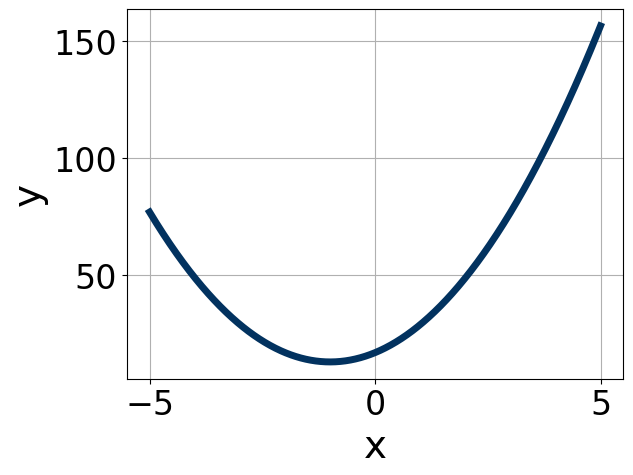
\includegraphics[width = 0.3\textwidth]{../Figures/quadraticEquationToGraphCopyAB.png}\item 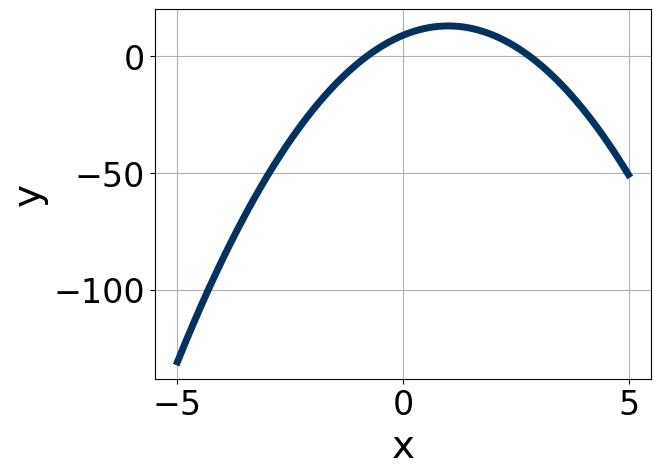
\includegraphics[width = 0.3\textwidth]{../Figures/quadraticEquationToGraphCopyBB.png}\item 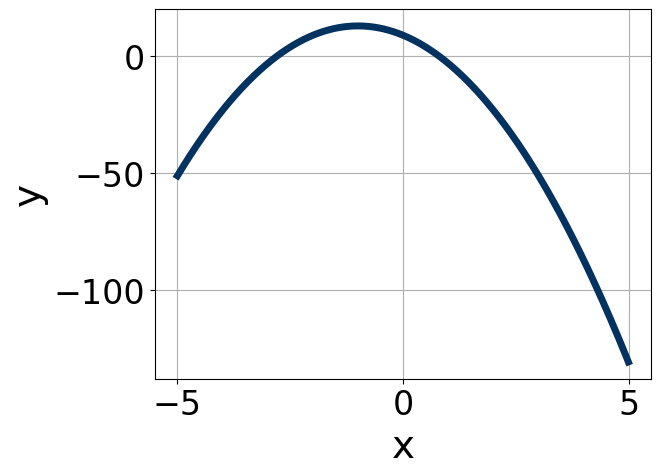
\includegraphics[width = 0.3\textwidth]{../Figures/quadraticEquationToGraphCopyCB.png}\item 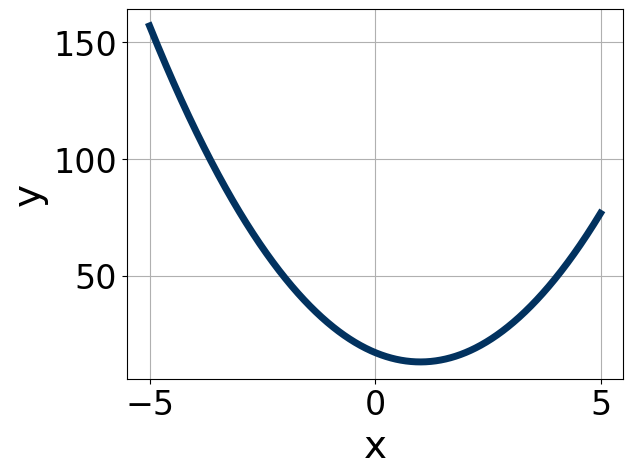
\includegraphics[width = 0.3\textwidth]{../Figures/quadraticEquationToGraphCopyDB.png}\end{multicols}\item None of the above.
\end{enumerate} }
\litem{
Graph the equation below.\[ f(x) = (x+3)^2 - 17 \]\begin{enumerate}[label=\Alph*.]
\begin{multicols}{2}\item 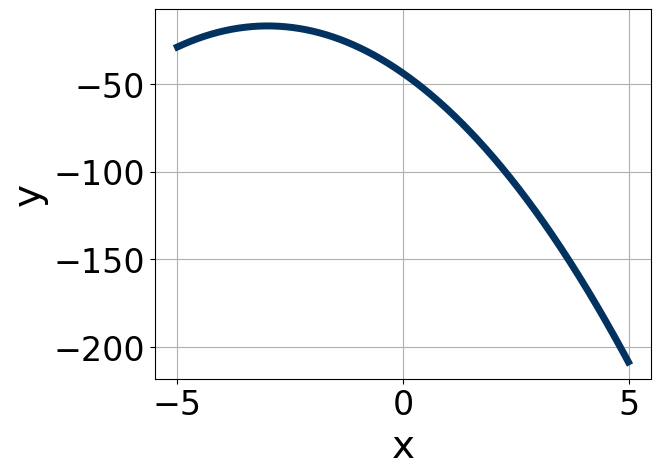
\includegraphics[width = 0.3\textwidth]{../Figures/quadraticEquationToGraphAB.png}\item 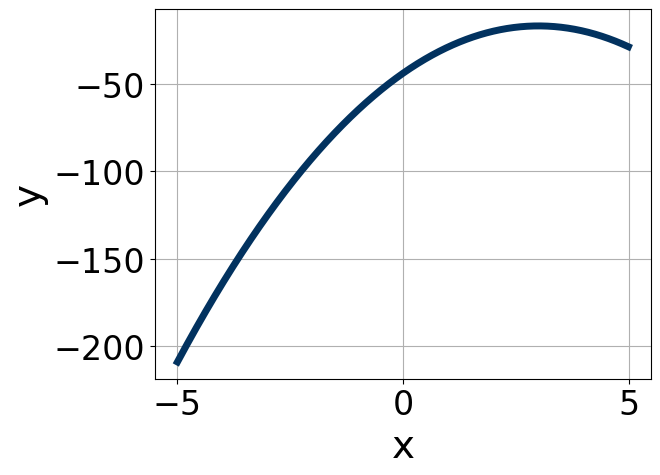
\includegraphics[width = 0.3\textwidth]{../Figures/quadraticEquationToGraphBB.png}\item 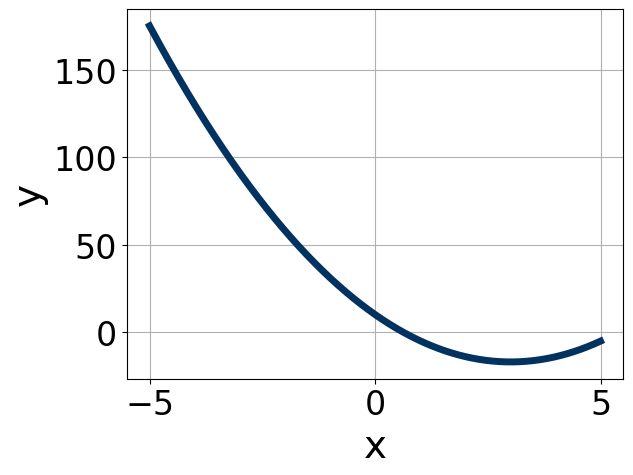
\includegraphics[width = 0.3\textwidth]{../Figures/quadraticEquationToGraphCB.png}\item 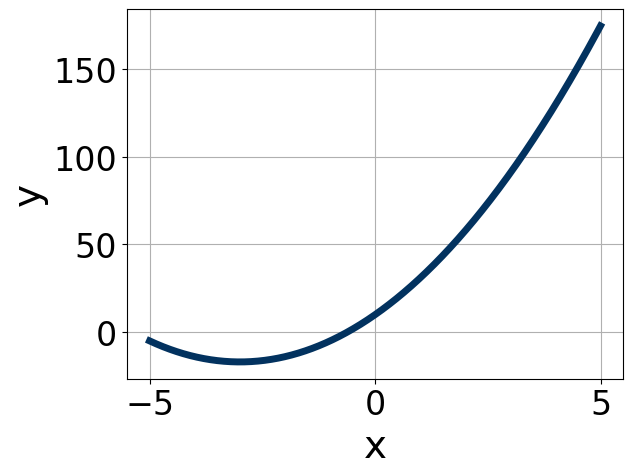
\includegraphics[width = 0.3\textwidth]{../Figures/quadraticEquationToGraphDB.png}\end{multicols}\item None of the above.
\end{enumerate} }
\litem{
Solve the quadratic equation below. Then, choose the intervals that the solutions $x_1$ and $x_2$ belong to, with $x_1 \leq x_2$.\[ 10x^{2} -33 x -54 = 0 \]\begin{enumerate}[label=\Alph*.]
\item \( x_1 \in [-1.56, -1] \text{ and } x_2 \in [4.25, 4.7] \)
\item \( x_1 \in [-4.03, -3.41] \text{ and } x_2 \in [1.41, 2.06] \)
\item \( x_1 \in [-6.05, -5.41] \text{ and } x_2 \in [0.5, 1.06] \)
\item \( x_1 \in [-12.11, -11.79] \text{ and } x_2 \in [44.85, 45.1] \)
\item \( x_1 \in [-0.64, -0.36] \text{ and } x_2 \in [12.88, 13.71] \)

\end{enumerate} }
\litem{
Write the equation of the graph presented below in the form $f(x)=ax^2+bx+c$, assuming  $a=1$ or $a=-1$. Then, choose the intervals that $a, b,$ and $c$ belong to.
\begin{center}
    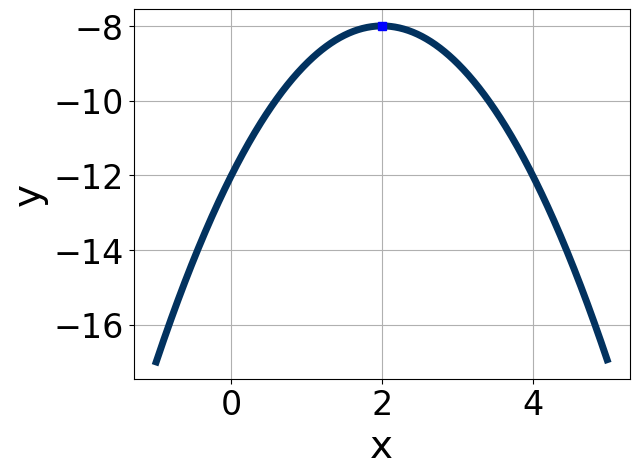
\includegraphics[width=0.5\textwidth]{../Figures/quadraticGraphToEquationCopyB.png}
\end{center}
\begin{enumerate}[label=\Alph*.]
\item \( a \in [0.2, 2.3], \hspace*{5mm} b \in [-7, -3], \text{ and } \hspace*{5mm} c \in [-6, -2] \)
\item \( a \in [-1.5, -0.4], \hspace*{5mm} b \in [2, 5], \text{ and } \hspace*{5mm} c \in [-14, -8] \)
\item \( a \in [-1.5, -0.4], \hspace*{5mm} b \in [-7, -3], \text{ and } \hspace*{5mm} c \in [-14, -8] \)
\item \( a \in [-1.5, -0.4], \hspace*{5mm} b \in [-7, -3], \text{ and } \hspace*{5mm} c \in [0, 6] \)
\item \( a \in [0.2, 2.3], \hspace*{5mm} b \in [2, 5], \text{ and } \hspace*{5mm} c \in [-6, -2] \)

\end{enumerate} }
\litem{
Factor the quadratic below. Then, choose the intervals that contain the constants in the form $(ax+b)(cx+d); b \leq d.$\[ 36x^{2} +60 x + 25 \]\begin{enumerate}[label=\Alph*.]
\item \( a \in [0.6, 1.05], \hspace*{5mm} b \in [27, 33], \hspace*{5mm} c \in [0.97, 1.13], \text{ and } \hspace*{5mm} d \in [26, 38] \)
\item \( a \in [2.43, 4.04], \hspace*{5mm} b \in [1, 10], \hspace*{5mm} c \in [11.16, 12.86], \text{ and } \hspace*{5mm} d \in [3, 6] \)
\item \( a \in [11.96, 12.5], \hspace*{5mm} b \in [1, 10], \hspace*{5mm} c \in [2.71, 3.3], \text{ and } \hspace*{5mm} d \in [3, 6] \)
\item \( a \in [5.99, 6.49], \hspace*{5mm} b \in [1, 10], \hspace*{5mm} c \in [4.07, 6.43], \text{ and } \hspace*{5mm} d \in [3, 6] \)
\item \( \text{None of the above.} \)

\end{enumerate} }
\litem{
Solve the quadratic equation below. Then, choose the intervals that the solutions $x_1$ and $x_2$ belong to, with $x_1 \leq x_2$.\[ 15x^{2} -2 x -24 = 0 \]\begin{enumerate}[label=\Alph*.]
\item \( x_1 \in [-0.97, -0.15] \text{ and } x_2 \in [3.89, 4.59] \)
\item \( x_1 \in [-6.31, -5.96] \text{ and } x_2 \in [0.04, 0.34] \)
\item \( x_1 \in [-18.67, -15.63] \text{ and } x_2 \in [19.39, 20.5] \)
\item \( x_1 \in [-3.62, -2.06] \text{ and } x_2 \in [0.51, 0.73] \)
\item \( x_1 \in [-2.36, -1.11] \text{ and } x_2 \in [1.03, 1.64] \)

\end{enumerate} }
\litem{
Factor the quadratic below. Then, choose the intervals that contain the constants in the form $(ax+b)(cx+d); b \leq d.$\[ 36x^{2} +60 x + 25 \]\begin{enumerate}[label=\Alph*.]
\item \( a \in [5.81, 7.04], \hspace*{5mm} b \in [-1, 8], \hspace*{5mm} c \in [5.74, 8.31], \text{ and } \hspace*{5mm} d \in [5, 6] \)
\item \( a \in [2.71, 4.49], \hspace*{5mm} b \in [-1, 8], \hspace*{5mm} c \in [11.27, 12.45], \text{ and } \hspace*{5mm} d \in [5, 6] \)
\item \( a \in [0.63, 1.49], \hspace*{5mm} b \in [26, 33], \hspace*{5mm} c \in [0.61, 1.01], \text{ and } \hspace*{5mm} d \in [28, 33] \)
\item \( a \in [16.36, 19.03], \hspace*{5mm} b \in [-1, 8], \hspace*{5mm} c \in [1.34, 3.05], \text{ and } \hspace*{5mm} d \in [5, 6] \)
\item \( \text{None of the above.} \)

\end{enumerate} }
\litem{
Solve the quadratic equation below. Then, choose the intervals that the solutions belong to, with $x_1 \leq x_2$ (if they exist).\[ -10x^{2} +15 x + 4 = 0 \]\begin{enumerate}[label=\Alph*.]
\item \( x_1 \in [-0.7, 1.2] \text{ and } x_2 \in [1, 2.1] \)
\item \( x_1 \in [-19.1, -18.1] \text{ and } x_2 \in [19, 21.8] \)
\item \( x_1 \in [-2.9, -0.4] \text{ and } x_2 \in [0.1, 0.9] \)
\item \( x_1 \in [-18.5, -16.1] \text{ and } x_2 \in [2.2, 3.1] \)
\item \( \text{There are no Real solutions.} \)

\end{enumerate} }
\litem{
Write the equation of the graph presented below in the form $f(x)=ax^2+bx+c$, assuming  $a=1$ or $a=-1$. Then, choose the intervals that $a, b,$ and $c$ belong to.
\begin{center}
    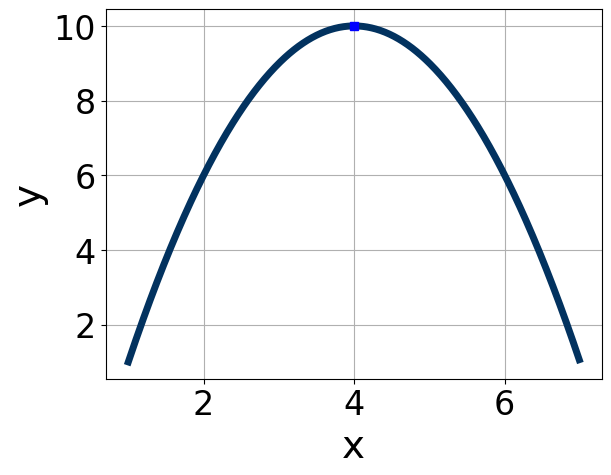
\includegraphics[width=0.5\textwidth]{../Figures/quadraticGraphToEquationB.png}
\end{center}
\begin{enumerate}[label=\Alph*.]
\item \( a \in [-2, 0], \hspace*{5mm} b \in [-8, -7], \text{ and } \hspace*{5mm} c \in [-6, -4] \)
\item \( a \in [0, 4], \hspace*{5mm} b \in [-8, -7], \text{ and } \hspace*{5mm} c \in [25, 27] \)
\item \( a \in [0, 4], \hspace*{5mm} b \in [7, 12], \text{ and } \hspace*{5mm} c \in [25, 27] \)
\item \( a \in [-2, 0], \hspace*{5mm} b \in [7, 12], \text{ and } \hspace*{5mm} c \in [-6, -4] \)
\item \( a \in [-2, 0], \hspace*{5mm} b \in [-8, -7], \text{ and } \hspace*{5mm} c \in [-28, -22] \)

\end{enumerate} }
\end{enumerate}

\end{document}